
%%%%%%%%%%%%%%%%%%%%%%%%%%%%%%%%%%%%%%%%%%%%%%%%%%%%%%%%%%%%%%%%%%%%%%%%%%%%%% 
\section{Detector configuration}

Configuration of the Mu2e detector is described by its subdetector configurations,
as shown in Figure~\ref{figure:configuration_top}.

For example, for the Mu2e tracker the levels of hierarchy look as follows:
tracker->stations->planes->panels.
Elements (substructures) are subdetector-specific, however element has
two mandatory fields: "enabled" and "status", used for configuration,
monitoring, and error reporting.

%%%%%%%%%%%%%%%%%%%%%%%%%%%%%%%%%%%%%%%%%%%%%%%%%%%%%%%%%%%%%%%%%%%%%%%%%%%%%% .

\subsubsection{Tracker} 


A top view of the tracker configuration
is shown in Figure~\ref{figure:tracker_config}.
\begin{itemize}
\item
  enabled = 0: the element (subtree) is considered present, but not used.
\item
  enabled = 1:
  \begin{itemize}
  \item
    status = 0 : the subsystem is OK
  \item
    status < 0 : the subsystem has a problem and an action is required
    The value of the status variable is the error code
  \item
    status > 0 : the subsystem has a warning-level problem, no immediate action
    is required
  \end{itemize}
\end{itemize}

\begin{figure}[H]
  \begin{tikzpicture}
    \node[anchor=south west,inner sep=0] at (0,0.) {
      % \node[shift={(0 cm,0.cm)},inner sep=0,rotate={90}] at (0,0) {}
      \makebox[\textwidth][c] {
        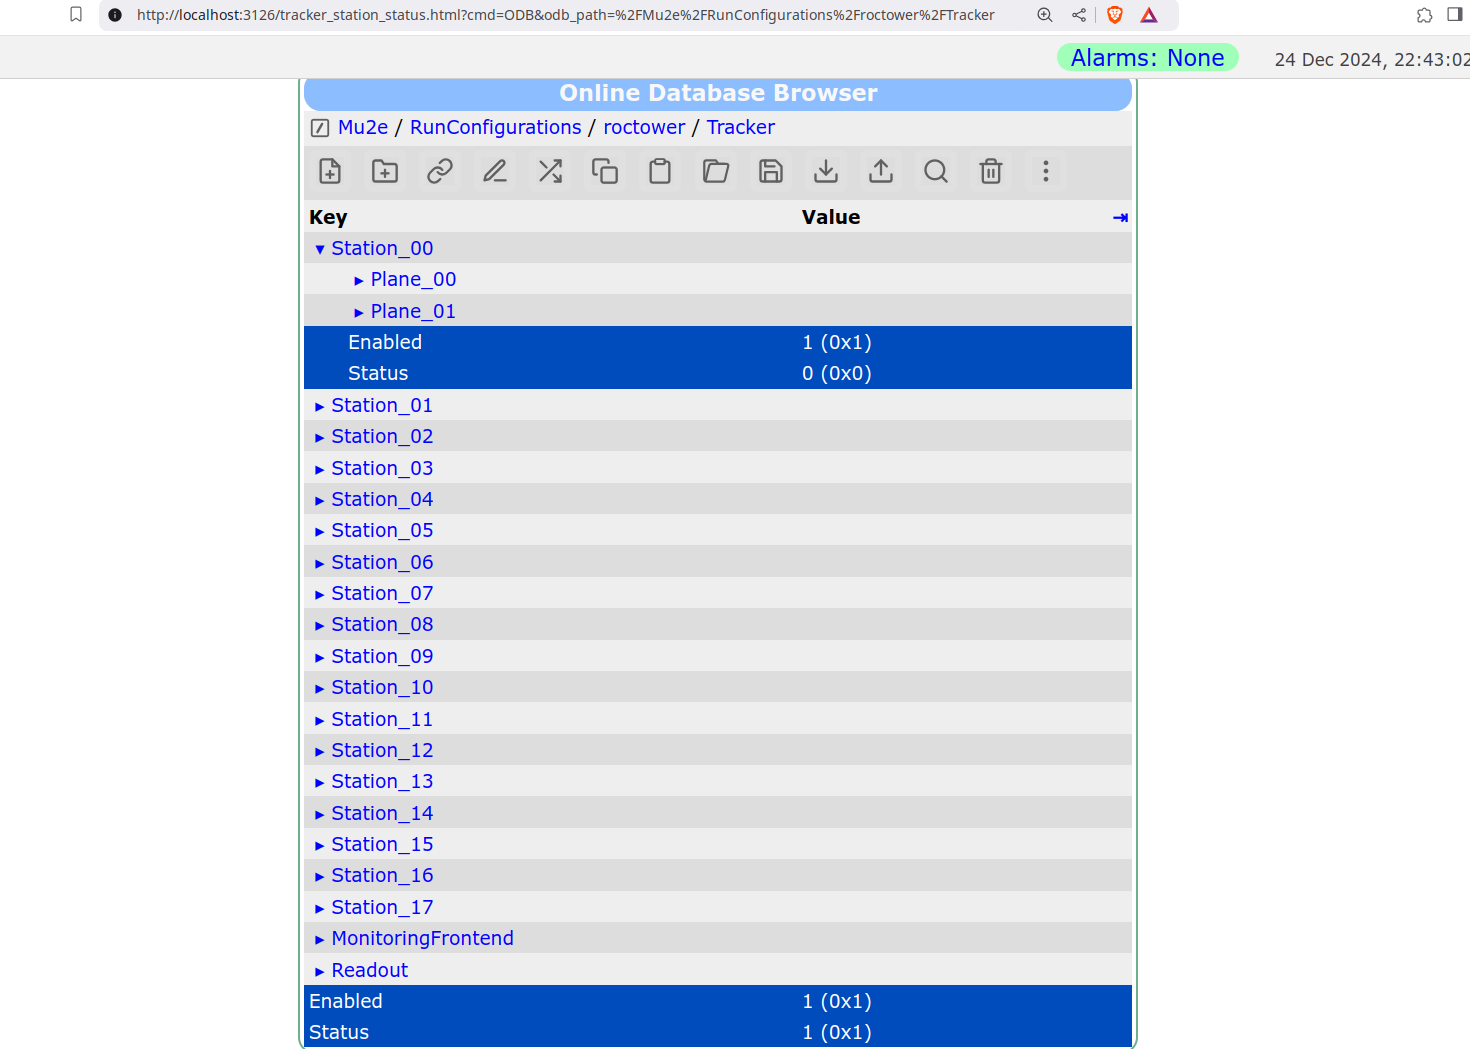
\includegraphics[width=0.95\textwidth]{png/tracker_config}
      }
    };
    % \node [text width=8cm, scale=1.0] at (14.5,0.5) {$\mu_B$, expected background mean};
    % \node [text width=8cm, scale=1.0, rotate={90}] at (1.5,7.5) { $S_{D}$, ``discovery'' signal strength  };
  \end{tikzpicture}
  \caption{
    \label{figure:tracker_config}
    Tracker: configuration levels from the station down to the panel, .
  }
\end{figure}


The next hierarchical levels of the tracker configuration, including the level of individual panels,
are shown in Figure~\ref{figure:station_config}.

\begin{figure}[H]
  \begin{tikzpicture}
    \node[anchor=south west,inner sep=0] at (0,0.) {
      % \node[shift={(0 cm,0.cm)},inner sep=0,rotate={90}] at (0,0) {}
      \makebox[\textwidth][c] {
        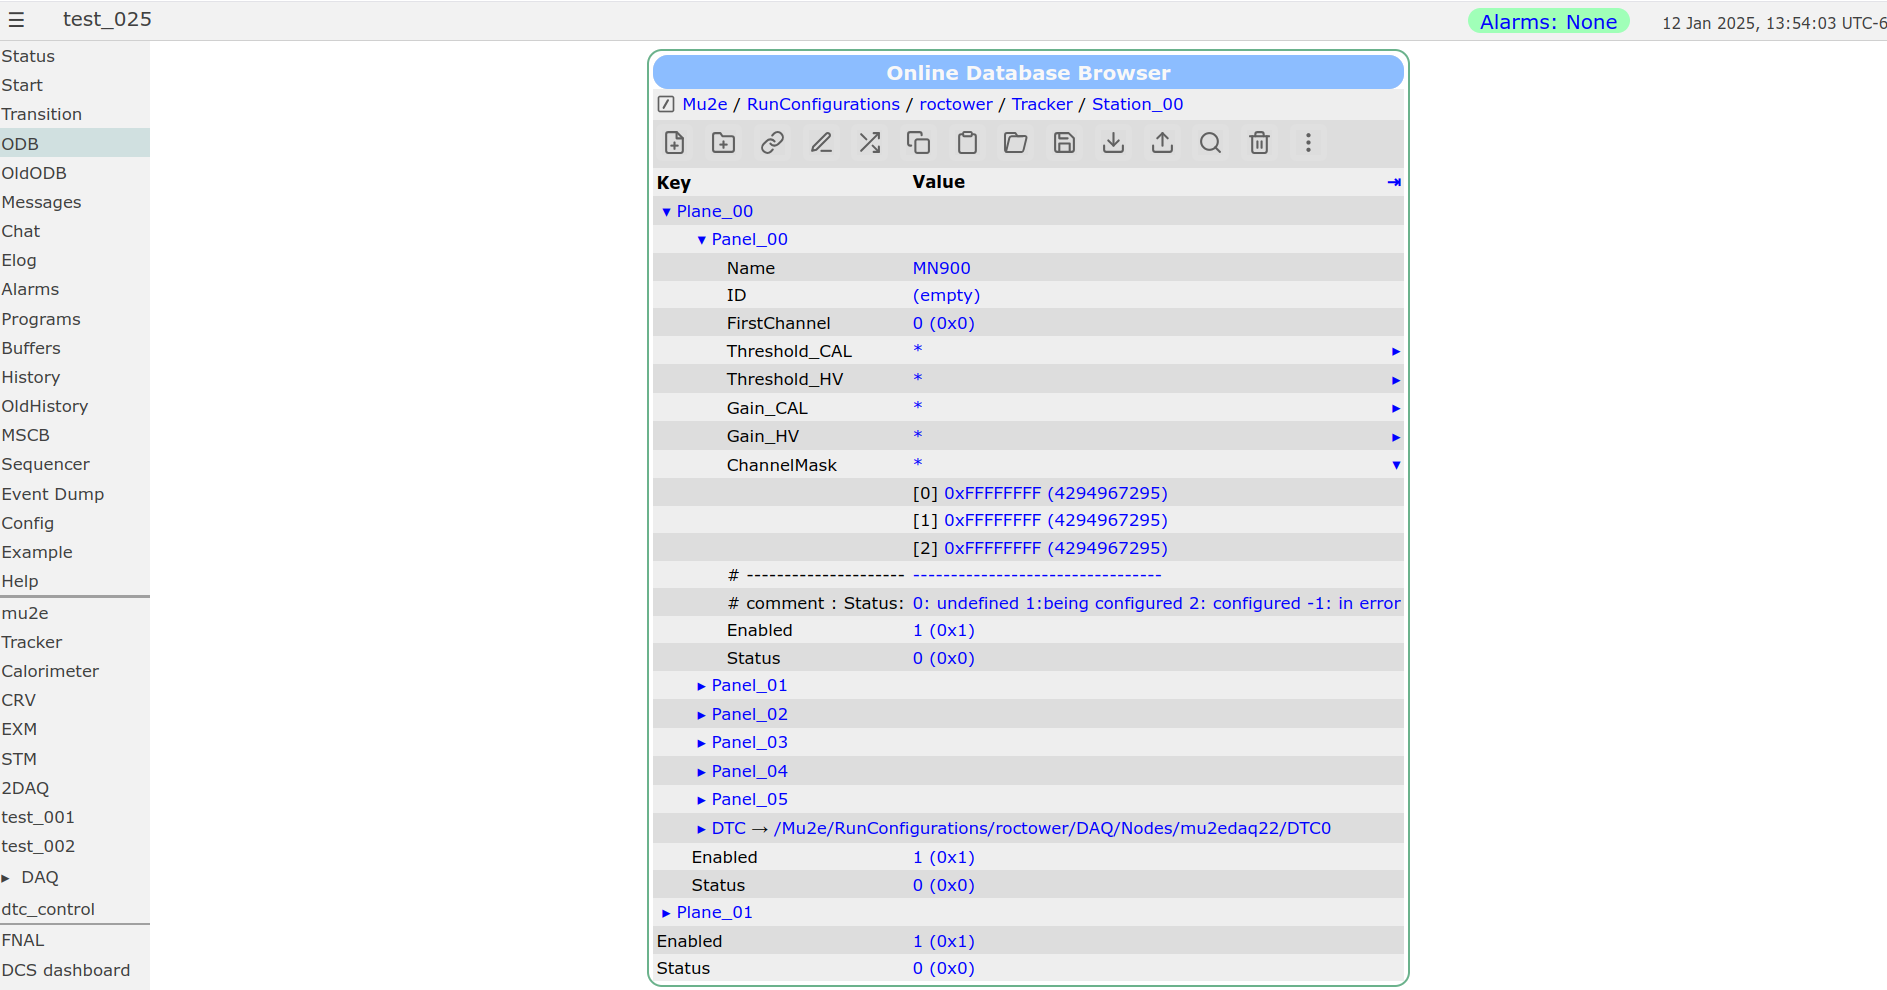
\includegraphics[width=0.95\textwidth]{png/station_config}
      }
    };
    % \node [text width=8cm, scale=1.0] at (14.5,0.5) {$\mu_B$, expected background mean};
    % \node [text width=8cm, scale=1.0, rotate={90}] at (1.5,7.5) { $S_{D}$, ``discovery'' signal strength  };
  \end{tikzpicture}
  \caption{
    \label{figure:station_config}
    Tracker configuration. The tracker, as well as each of the stations, has ``Enabled'' and
    ``Status'' fields.
  }
\end{figure}

%%%%%%%%%%%%%%%%%%%%%%%%%%%%%%%%%%%%%%%%%%%%%%%%%%%%%%%%%%%%%%%%%%%%%%%%%%%%%% 
\subsection{Calorimeter} 


%%%%%%%%%%%%%%%%%%%%%%%%%%%%%%%%%%%%%%%%%%%%%%%%%%%%%%%%%%%%%%%%%%%%%%%%%%%%%% 
\subsection{CRV} 


%%%%%%%%%%%%%%%%%%%%%%%%%%%%%%%%%%%%%%%%%%%%%%%%%%%%%%%%%%%%%%%%%%%%%%%%%%%%%% 
\subsection{STM} 




%%% Local Variables:
%%% mode: latex
%%% TeX-master: t
%%% End:
